\documentclass[10pt]{article}
\usepackage[margin=0.64in]{geometry}
\usepackage[T1]{fontenc}
\usepackage{lmodern,amsmath,amssymb,graphicx,booktabs,hyperref,array}
\hypersetup{colorlinks=true,urlcolor=blue}
\setlength{\parindent}{0pt}
\setlength{\parskip}{5pt}
\pagestyle{plain}
\newcommand{\uv}{\texttt{[pcc:unverified]}}
\begin{document}
\begin{center}
{\Large Public-input multiplier roots and geometric rows}\\[3pt]
{\small Curve25519 native correctness component --- 24 November 2026}
\end{center}
\textbf{Result.} Each original-field control---public raw $u=9$, its negative,
and a known-consistent raw target---returns four checked multiplier lifts but
one normalized geometric signed row. All 96 admitted toy raw targets match
complete direct enumeration, including 38 zero-result targets. This is
adapted-base pair correctness, with producer-unsigned evidence. \texttt{[pcc:unverified]}

\textbf{Input and domain.} The public query receives only \texttt{Spec}, raw
$R$ and a work cap. It derives templates $h,h^2$ internally; no known
$\sigma$, scalar, point tuple, candidate list or supplied section enters
\texttt{solve()}. Original parameters are
$p=2^{255}-19$, $A=486662$, $a=60824497$, $q=213156431$, $K=20633$,
with the original $h$. Output has relative labels $(1,0),(2,0)$ in the adapted
base $S_\sigma$, raw sum $R$, and image sum $Q=[8]R$. The finite raw-$R$
sector requires nonidentity $Q$. Full prime-target coverage needs eight torsion
translates or a separate sector argument. \texttt{[pcc:unverified]}

\begin{center}
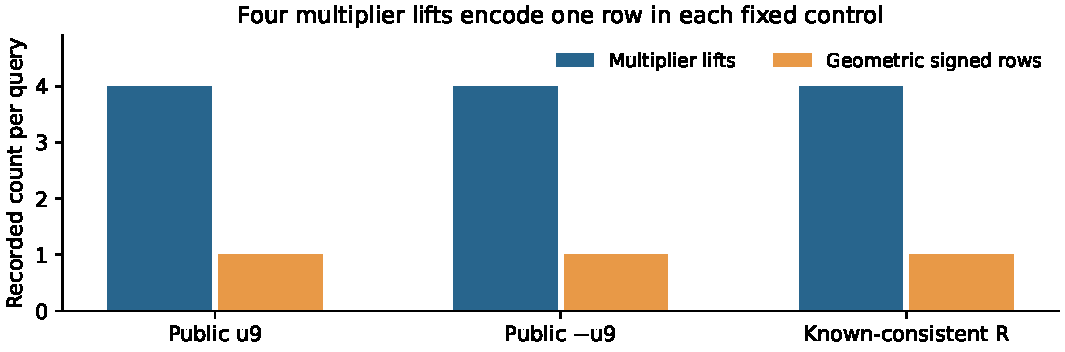
\includegraphics[width=0.88\linewidth]{counts.pdf}\\[-2pt]
{\footnotesize Recorded fixed controls, native revision 2; $+u9/-u9$ are related.
No random-target yield or statistical uncertainty is estimated.}
\end{center}
\vspace{-5pt}
\begin{center}\small
\begin{tabular}{lrrrr}
\toprule
Query & Branch degrees & Finite candidates & Infinity lifts & Lifts / rows\\
\midrule
Public $u9$ & $8,8,8,8$ & 4 & 0 & 4 / 1\\
Public $-u9$ & $8,8,8,8$ & 4 & 0 & 4 / 1\\
Known-consistent $R$ & $8,8,8,7$ & 3 & 1 & 4 / 1\\
\bottomrule
\end{tabular}\end{center}

\textbf{Toy completeness and flow.} For
$p=101,A=95,a=17,q=3,K=8,h=(17,12)$, the direct reference enumerates all
102 torus parameters, including the infinity chart. All 96 admitted finite
raw targets agree as complete ordered multiplier/raw-pair sets: 284 lifts,
two infinity lifts and 46 distinct geometric rows across the stream. Seven
finite cofactor-torsion targets are outside admission. The direct reference
shares field/group primitives, so it is separate from the root path but is
not independent signed native verification. \texttt{[pcc:unverified]}

The single fixed call completed all four planned groups with zero failed
groups, 110 records, 99 queries (96 toy plus three actual) and exit 0.
Fourteen refusals include three changed-lift cases. Four release unit tests,
formatting, strict all-target Clippy and build passed before qualification.
Forced caps and unsupported zero-polynomial cases remain incomplete errors,
never absence certificates. No qualified source changed or reran afterward. \texttt{[pcc:unverified]}

\textbf{Costs retained at their scope.} Partial new polynomial Engine counters
record 287978 Fp2 multiplications per public $\pm u9$ query and 263677 for the
known control. Group/spec/class-key work, allocation and complete cold costs
are unpriced; cumulative coefficient reservations are not peak RAM. No timing,
GAE, speed, fitted exponent or fastest-tool comparison is claimed. \texttt{[pcc:unverified]}

\newpage
\begin{center}{\large Construction, fidelity and next recovery gate}\end{center}
\begin{center}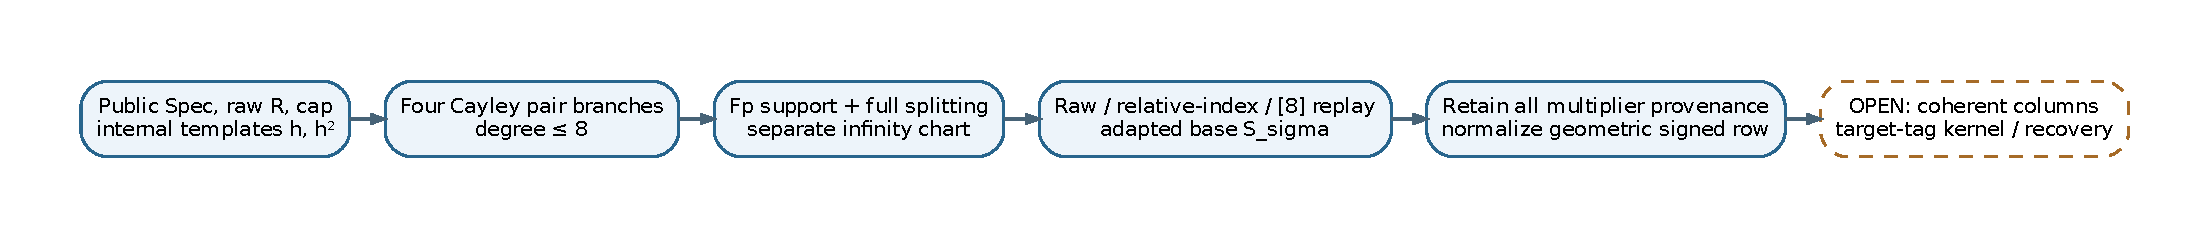
\includegraphics[width=\linewidth]{diagram.pdf}\end{center}

\textbf{Compiler and root support.} With $\sigma=(1+c\sqrt2)/(1-c\sqrt2)$,
$V=1-2c^2$, and $\alpha_i=h^i$, define
\[
 U_i=\alpha_{i,a}(1+2c^2)+4\alpha_{i,b}c,\qquad
 N_i=A(\epsilon_iV-U_i),\quad D_i=2U_i,\quad Z=D_1D_2.
\]
The denominator-cleared pair numerator at target abscissa $r$ is
\[
 (N_1D_2-N_2D_1)^2r^2
 -2\big((N_1D_2+N_2D_1)(N_1N_2+Z)+2AN_1N_2Z\big)r
 +(N_1N_2-Z)^2.
\]
Four sign branches have degree at most eight. The unchanged native arithmetic
Engine supplies field operations; a separate degree-eight adapter computes
$\gcd(P,X^p-X)$ and bounded complete splitting, then checks factor product
and multiplicities. The older degree-six Ring cap was not raised.
$\sigma=-1$ is handled separately. Rational raw lifts must satisfy the exact
relative map, raw sum and eightfold group sum. \texttt{[pcc:unverified]}

\textbf{Admission fidelity.} The original adapter requires a unique rational
branch \emph{before} zero/torsion filtering. Toy $z=\pm1$ has two rational
branches, including one with ordinate zero. Initial unpublished source counted
only after filtering; that source and passing development logs are retained.
Both constructor and external lift validator were corrected before the primary
call, with dedicated ambiguous-boundary controls. The shifted output is not an
unchanged full point-Circuit witness or a formal shifted compiler theorem. \texttt{[pcc:unverified]}

\textbf{Why the row count differs.} Negation swaps raw branches; inversion of
a norm-one parameter keeps its real coordinate. For $h,h^2$,
$\sigma'=h^{-3}\sigma^{-1}$ swaps the inverses of the two shifted parameters.
The known-target control explicitly finds the same geometric row at
$\sigma=1,-1,h^{-3}$. All actual cases retain four $\sigma^q$ parameter-base
keys but one row. This explains pair-row aliases; it does not equate the full
$K=20633$ bases or prove a general group action. \texttt{[pcc:unverified]}

\textbf{Next discriminator.} Freeze a coherent common-column or logarithm-
transport mechanism before six-leaf scaling. Retain raw/cofactor provenance,
form $Mz=a+bx$, and require $v^TM=0$ with $v^Tb\ne0$, followed by held-out scalar
replay. Private columns, repeated rows and sign/reciprocal relabels are negative
controls. This target-tag kernel/recovery gate is unimplemented. A free-base
degree bound supplies no common-base decomposition exponent. \texttt{[pcc:unverified]}

\textbf{Evidence and versions.} Native statement
\texttt{PCC-20261124-f08530} pins 18 subjects. Revision-2 source
\texttt{121d58164e} was published as \texttt{c224297669} before the call;
only main/wrapper transport differs from retained revision 1. Current
\texttt{SOURCES\_V2.sha256} has 103 inputs in four constituent archives,
with six compiled-in hashes matched. Full raw is 319552 bytes in one 20224-byte
lossless archive. Binary SHA-256 prefix \texttt{d72fa3da445facaafff8}; write-once
build/pre/post and actual positive/collision transport are retained. \texttt{[pcc:unverified]}

\textbf{Proof and literature scope.} Evaluated identity
\texttt{IDC1h54f6e499a51d5042} checks degree-10 homogeneous denominator
clearing at 32+32 points over $2^{61}-1$ with plus-one refusal; no formal
actual-field/compiler/group theorem follows. See \texttt{PROOF\_MAP.md},
\texttt{FIDELITY.md}, \texttt{SYMMETRY.md}, full \texttt{report.md} and
the frozen proposal's \texttt{SOURCES.md}: EFD Montgomery formulas,
Yokoyama et al. Proposition 1, official FLINT factoring, and scoped
Milne/Farashahi references. KB wrapper unavailable; prior Semaev PDF access
gap retained. Classical Semaev/Cayley/factoring carries no novelty claim.
Canonical performance graphs remain unchanged: no admitted performance row. \texttt{[pcc:unverified]}
\end{document}
